\chapter{Plan de pruebas}

\section{Visión general}

Durante el desarrollo del proyecto se han realizado diversas pruebas para asegurar la fiabilidad del sistema en completo, tratando de minimizar el número de fallos que pueden ocurrir. En este capítulo se van a explicar algunas de las pruebas realizadas.

\section{Pruebas del servidor OAI-PMH}

Además de haber realizado las rutinarias pruebas unitarias, para comprobar que el servidor genera respuestas \acrshort{xml} válidas ajustandose a la especificación del protocolo \acrshort{oaipmh}, se ha optado por utilizar una herramienta web que facilita esta verificación, el \acrshort{oaipmh} validator.

Se han realizado las siguientes pruebas mediante el uso de esta herramienta que verifica que el servidor funciona correctamente y por tanto los clientes que realicen las peticiones reciben las respuestas apropiadas:

\subsection{Verificación del comando Idenfity}

En esta comprobación se ha copiado la respuesta generada por el servidor \acrshort{oaipmh} a la petición \textit{Identify}. Como se puede ver en la figura \ref{fig:identify}, el validador ha comprobado que el documento \acrshort{xml} es válido, que cumple con el esquema de la versión 2.0 del protocolo y que la dirección del correo electrónico dispuesto para facilitar el soporte a incidencias es correcto.

\begin{figure}[!htbp]
	\centering
	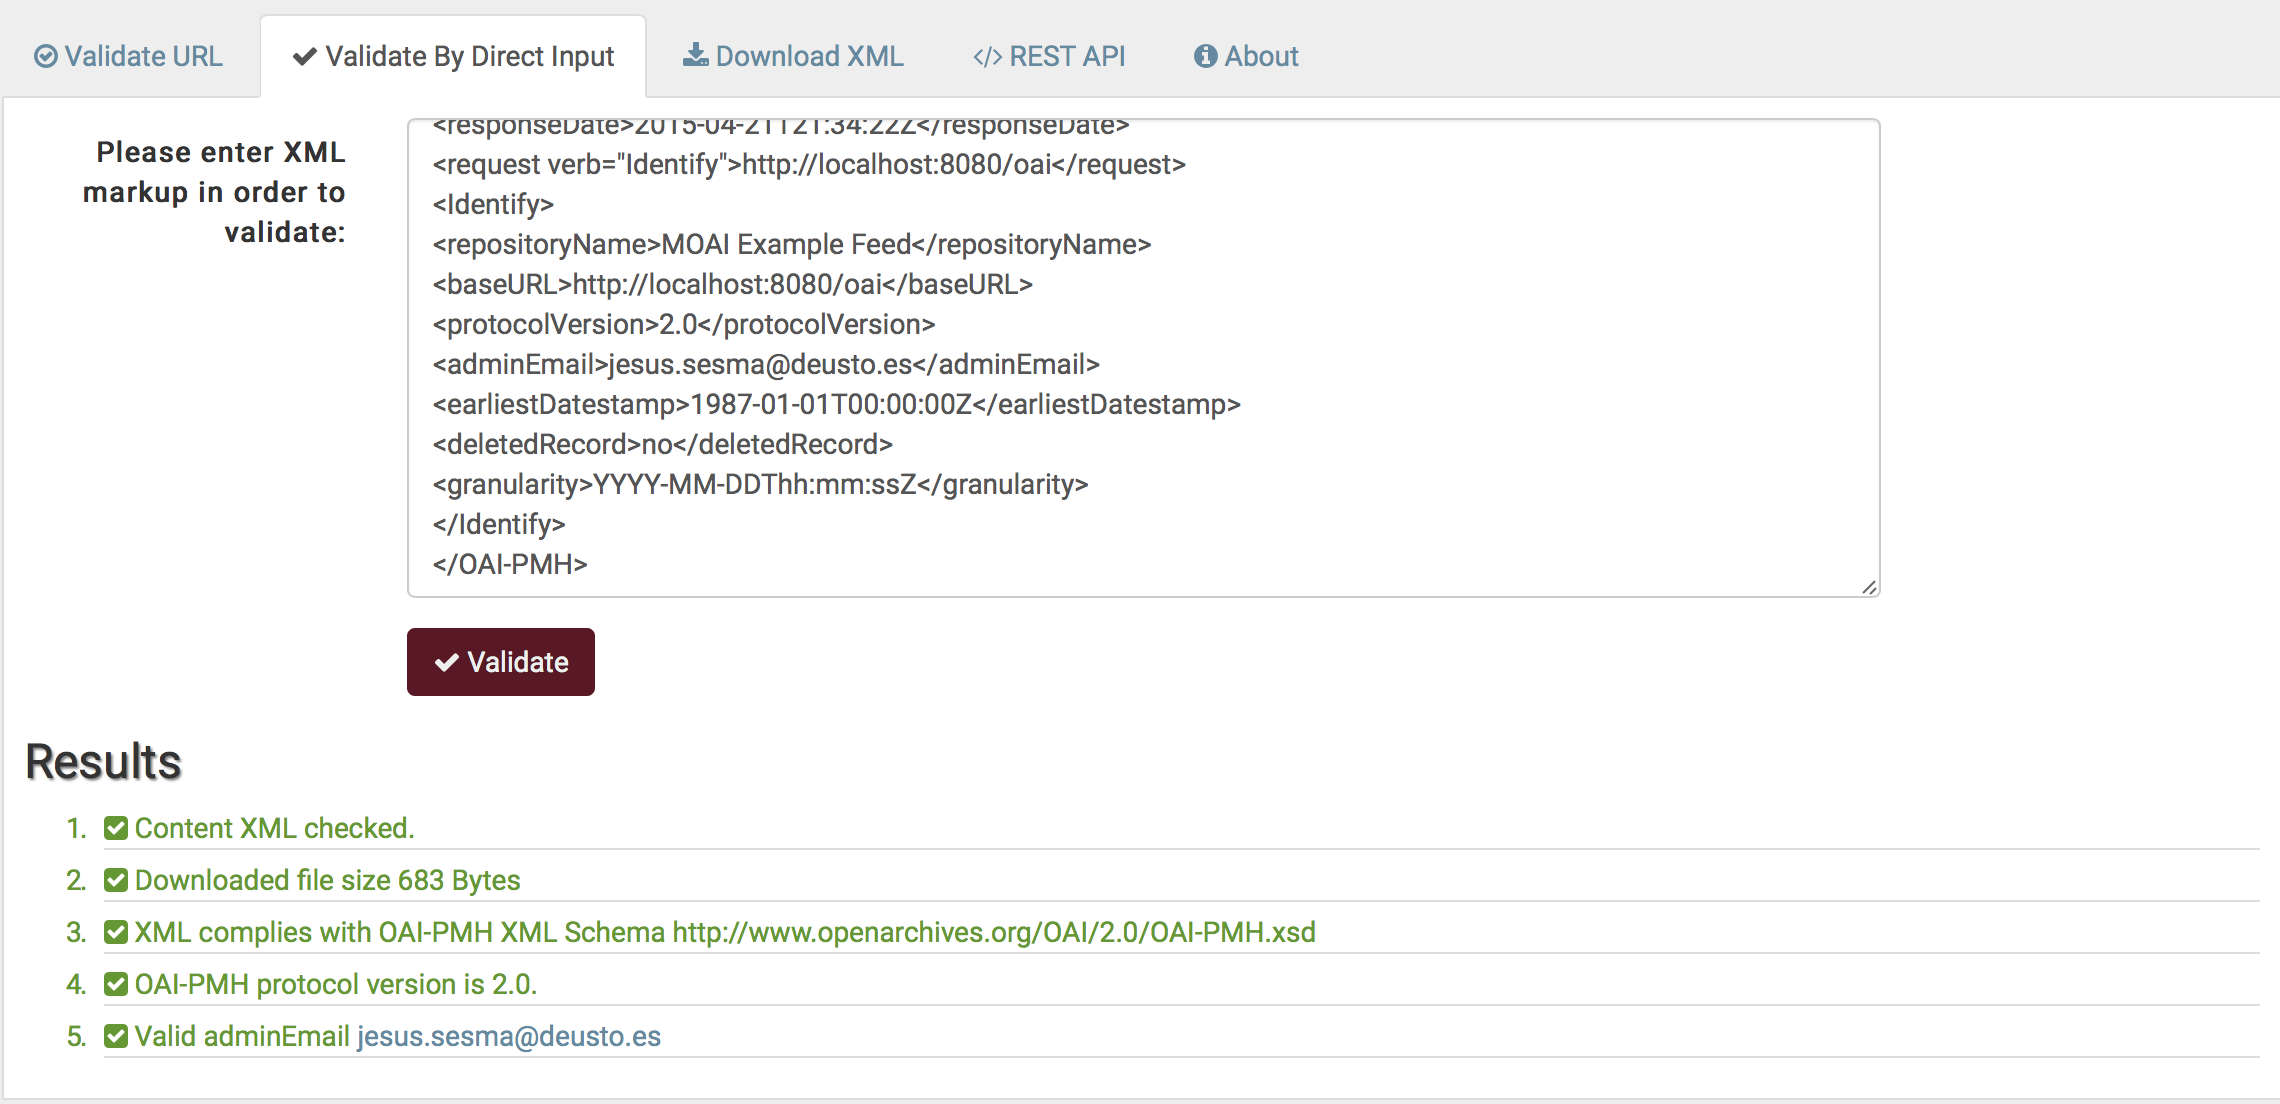
\includegraphics[scale=0.32]{fig/oaipmh_validations/Identify}
	\caption{Validación satisfactoria del comando Identify}
	\label{fig:identify}
\end{figure}

\subsection{Verificación del comando ListMetadataFormats}

En esta comprobación se ha copiado la respuesta generada por el servidor \acrshort{oaipmh} a la petición \textit{ListMetadataFormats}. Como se puede ver en la figura \ref{fig:listmetadataformats}, el validador ha comprobado que el documento \acrshort{xml} es válido, que cumple con el esquema de la versión 2.0 del protocolo. Por último lista los esquemas que soporta el servidor \acrshort{oaipmh}, siendo el primero de estos \acrlong{dc}, el formato bibliográfico estándar de soporte obligatorio, y el segundo un esquema opcional \acrfull{mods}\cite{MODS}.

\begin{figure}[!htbp]
	\centering
	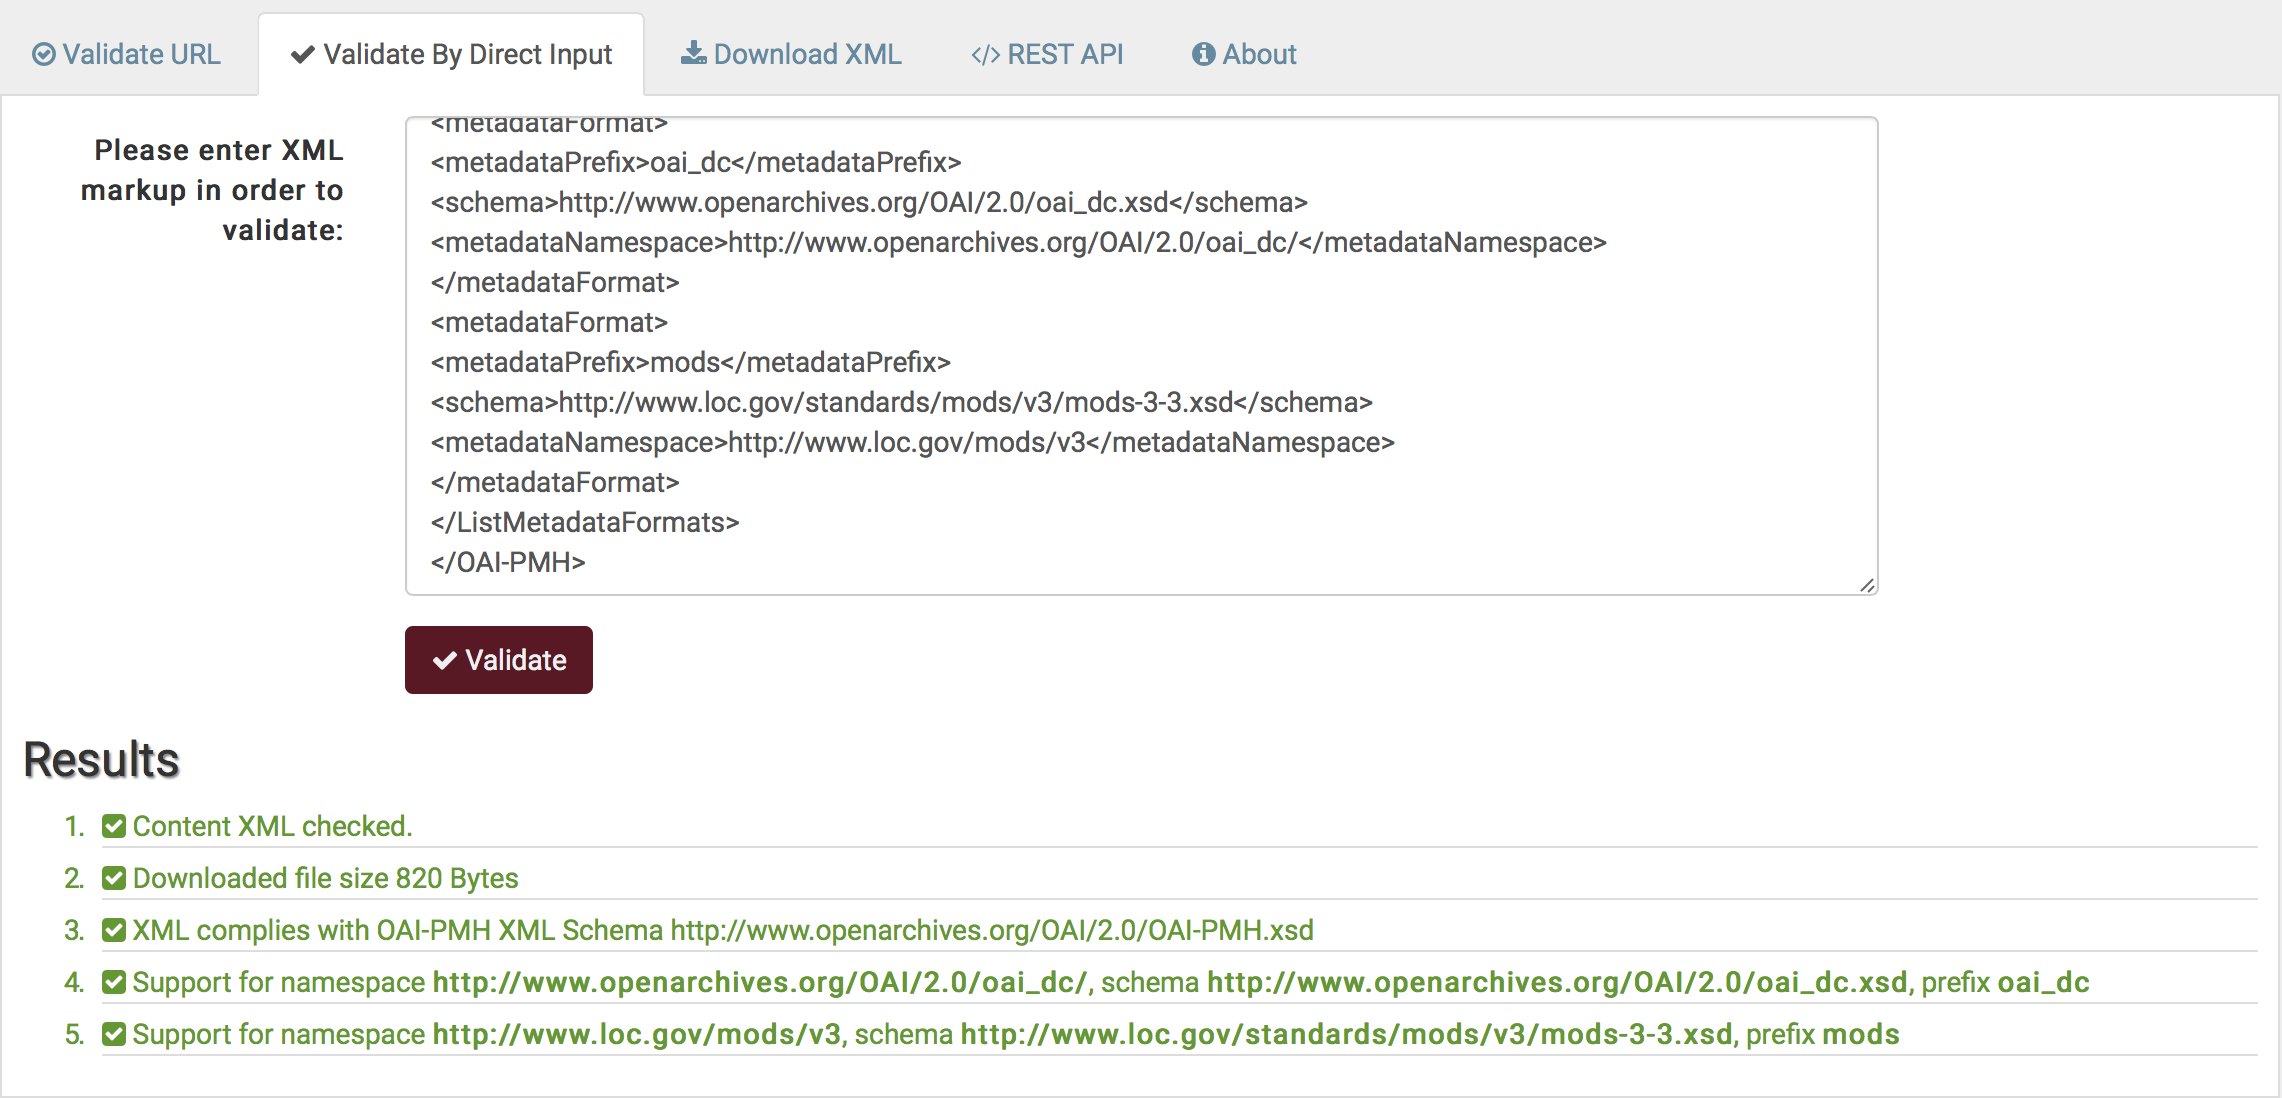
\includegraphics[scale=0.31]{fig/oaipmh_validations/ListMetadataFormats}
	\caption{Validación satisfactoria del comando ListMetadataFormats}
	\label{fig:listmetadataformats}
\end{figure}

\subsection{Verificación del comando ListSets}

En esta comprobación se ha copiado la respuesta generada por el servidor \acrshort{oaipmh} a la petición \textit{ListSets}. 

\begin{figure}[!htbp]
	\centering
	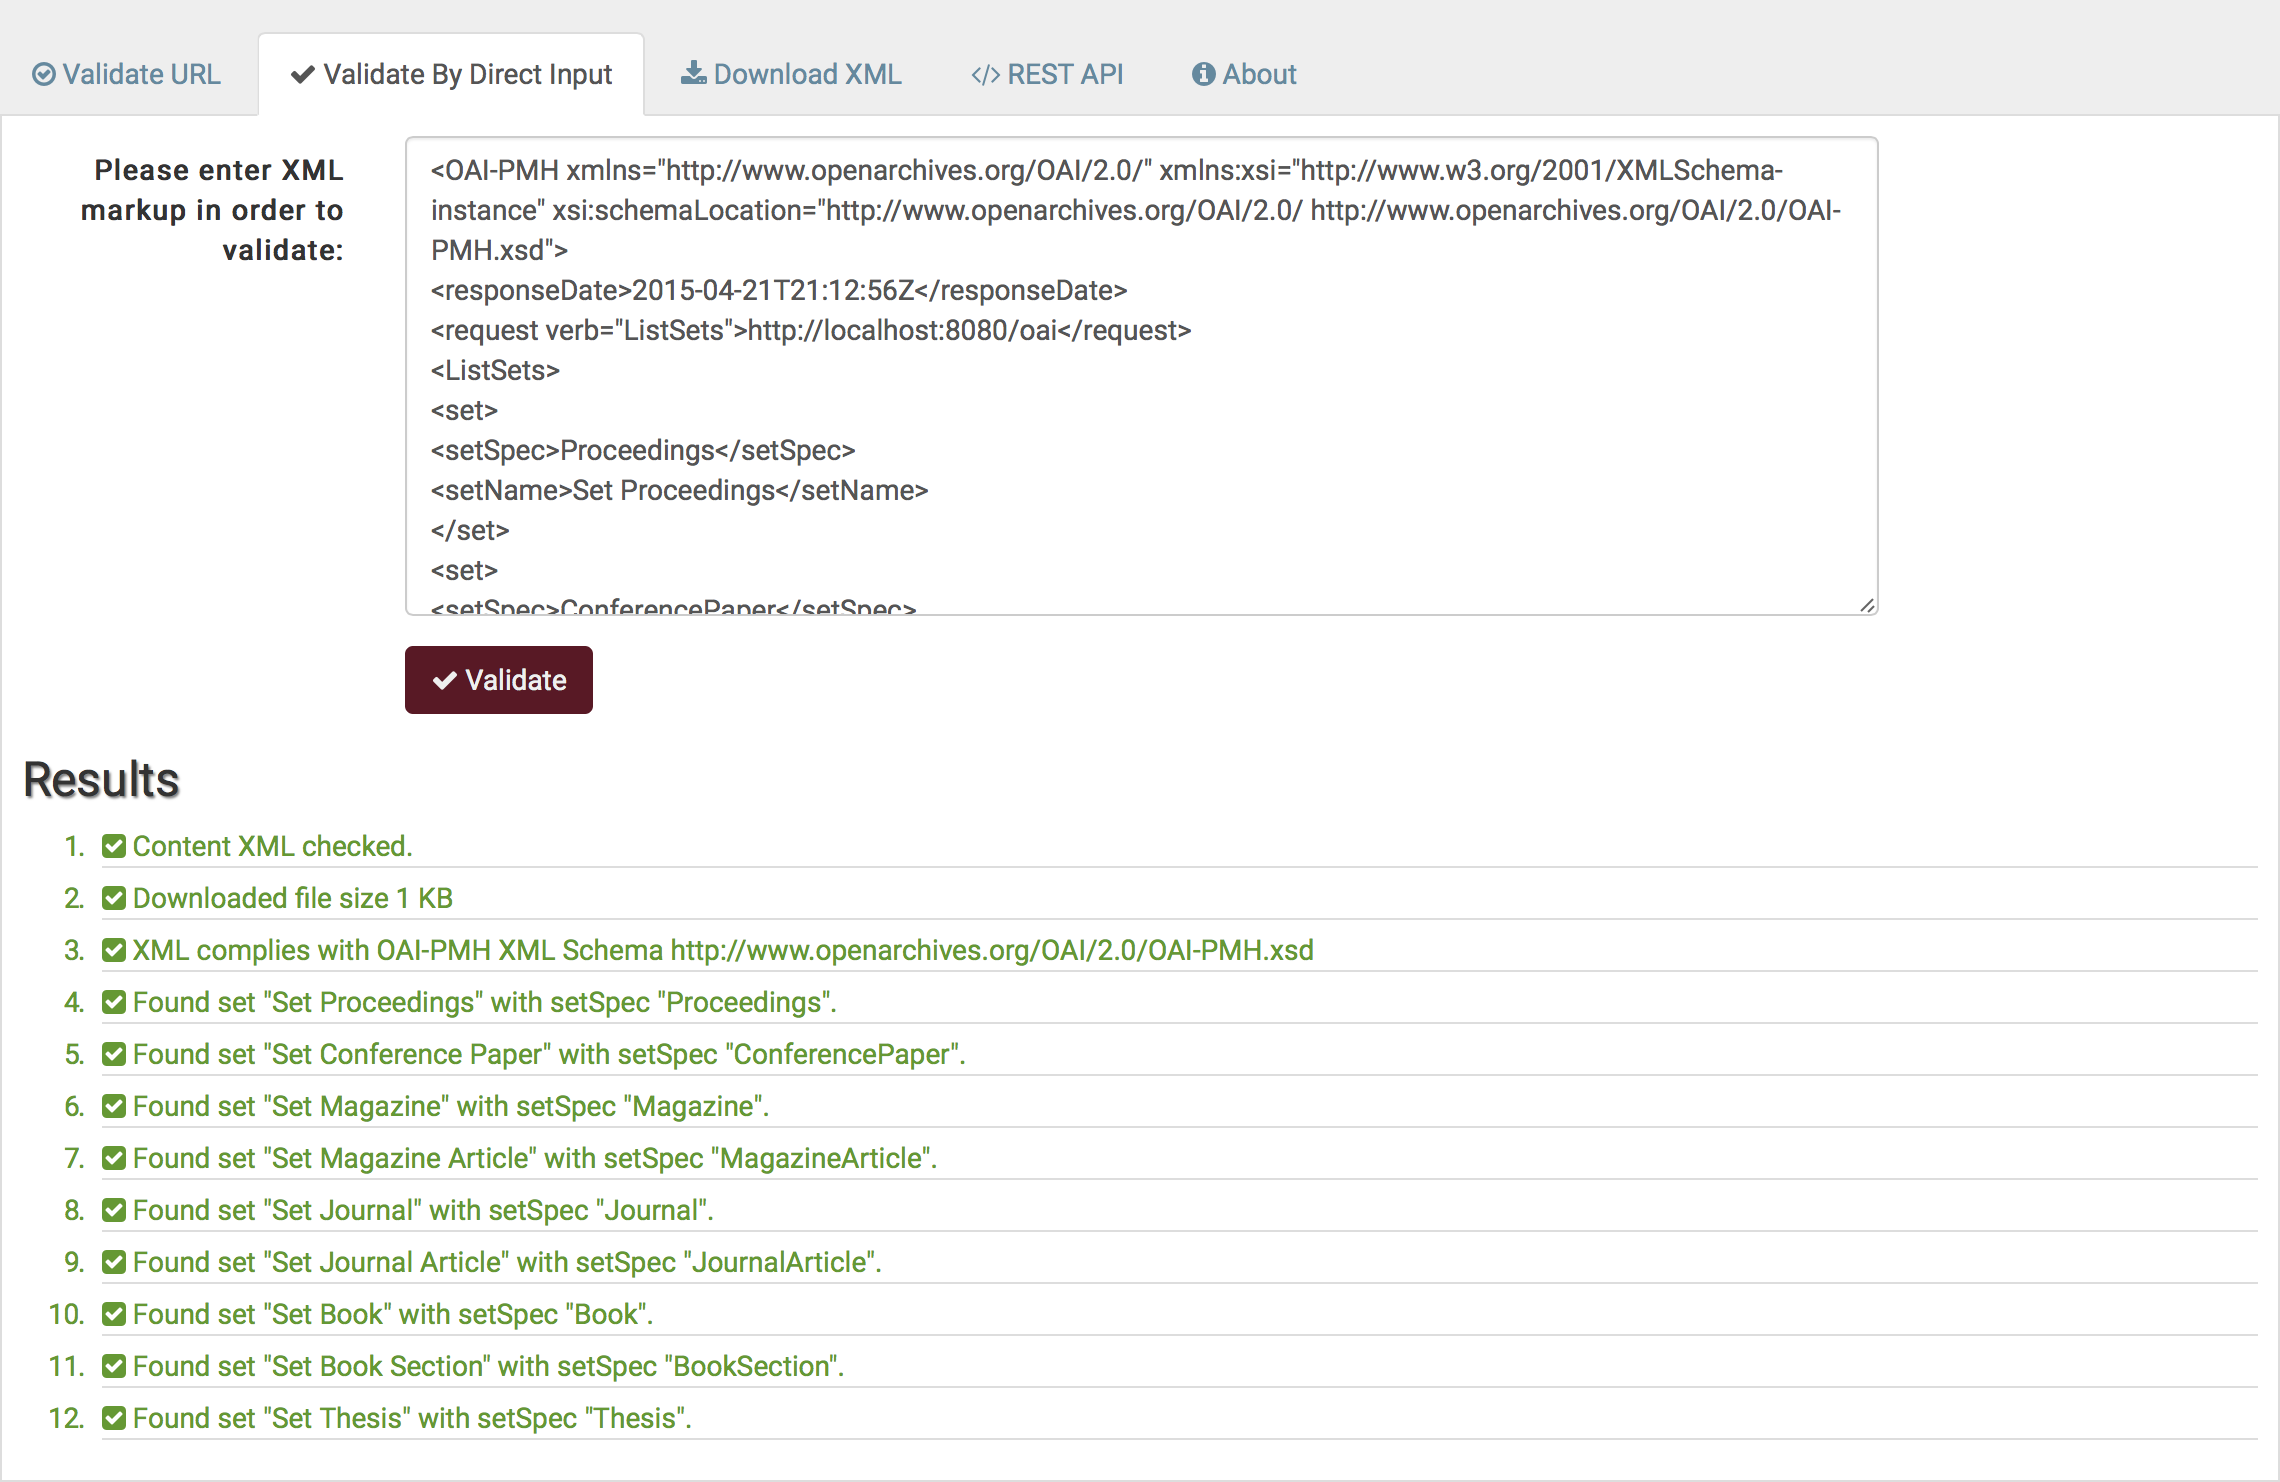
\includegraphics[scale=0.31]{fig/oaipmh_validations/ListSets}
	\caption{Validación satisfactoria del comando ListSets}
	\label{fig:listsets}
\end{figure}

Como se puede ver en la figura \ref{fig:listsets}, el validador ha comprobado que el documento \acrshort{xml} es válido, que cumple con el esquema de la versión 2.0 del protocolo. Por último lista los \textit{sets} opcionales que soporta el servidor \acrshort{oaipmh} para facilitar la recuperación selectiva de metadatos, siendo estos cada uno de los tipos de publicaciones disponibles en el repositorio de \acrshort{labman}.

\subsection{Verificación del comando ListIdentifiers}

En esta comprobación se ha copiado la respuesta generada por el servidor \acrshort{oaipmh} a las peticiones \textit{ListIdentifiers} y \textit{ListRecords}. Como se puede ver en la figura \ref{fig:listidentifiers}, el validador ha comprobado que el documento \acrshort{xml} es válido, que cumple con el esquema de la versión 2.0 del protocolo.

\begin{figure}[!htbp]
	\centering
	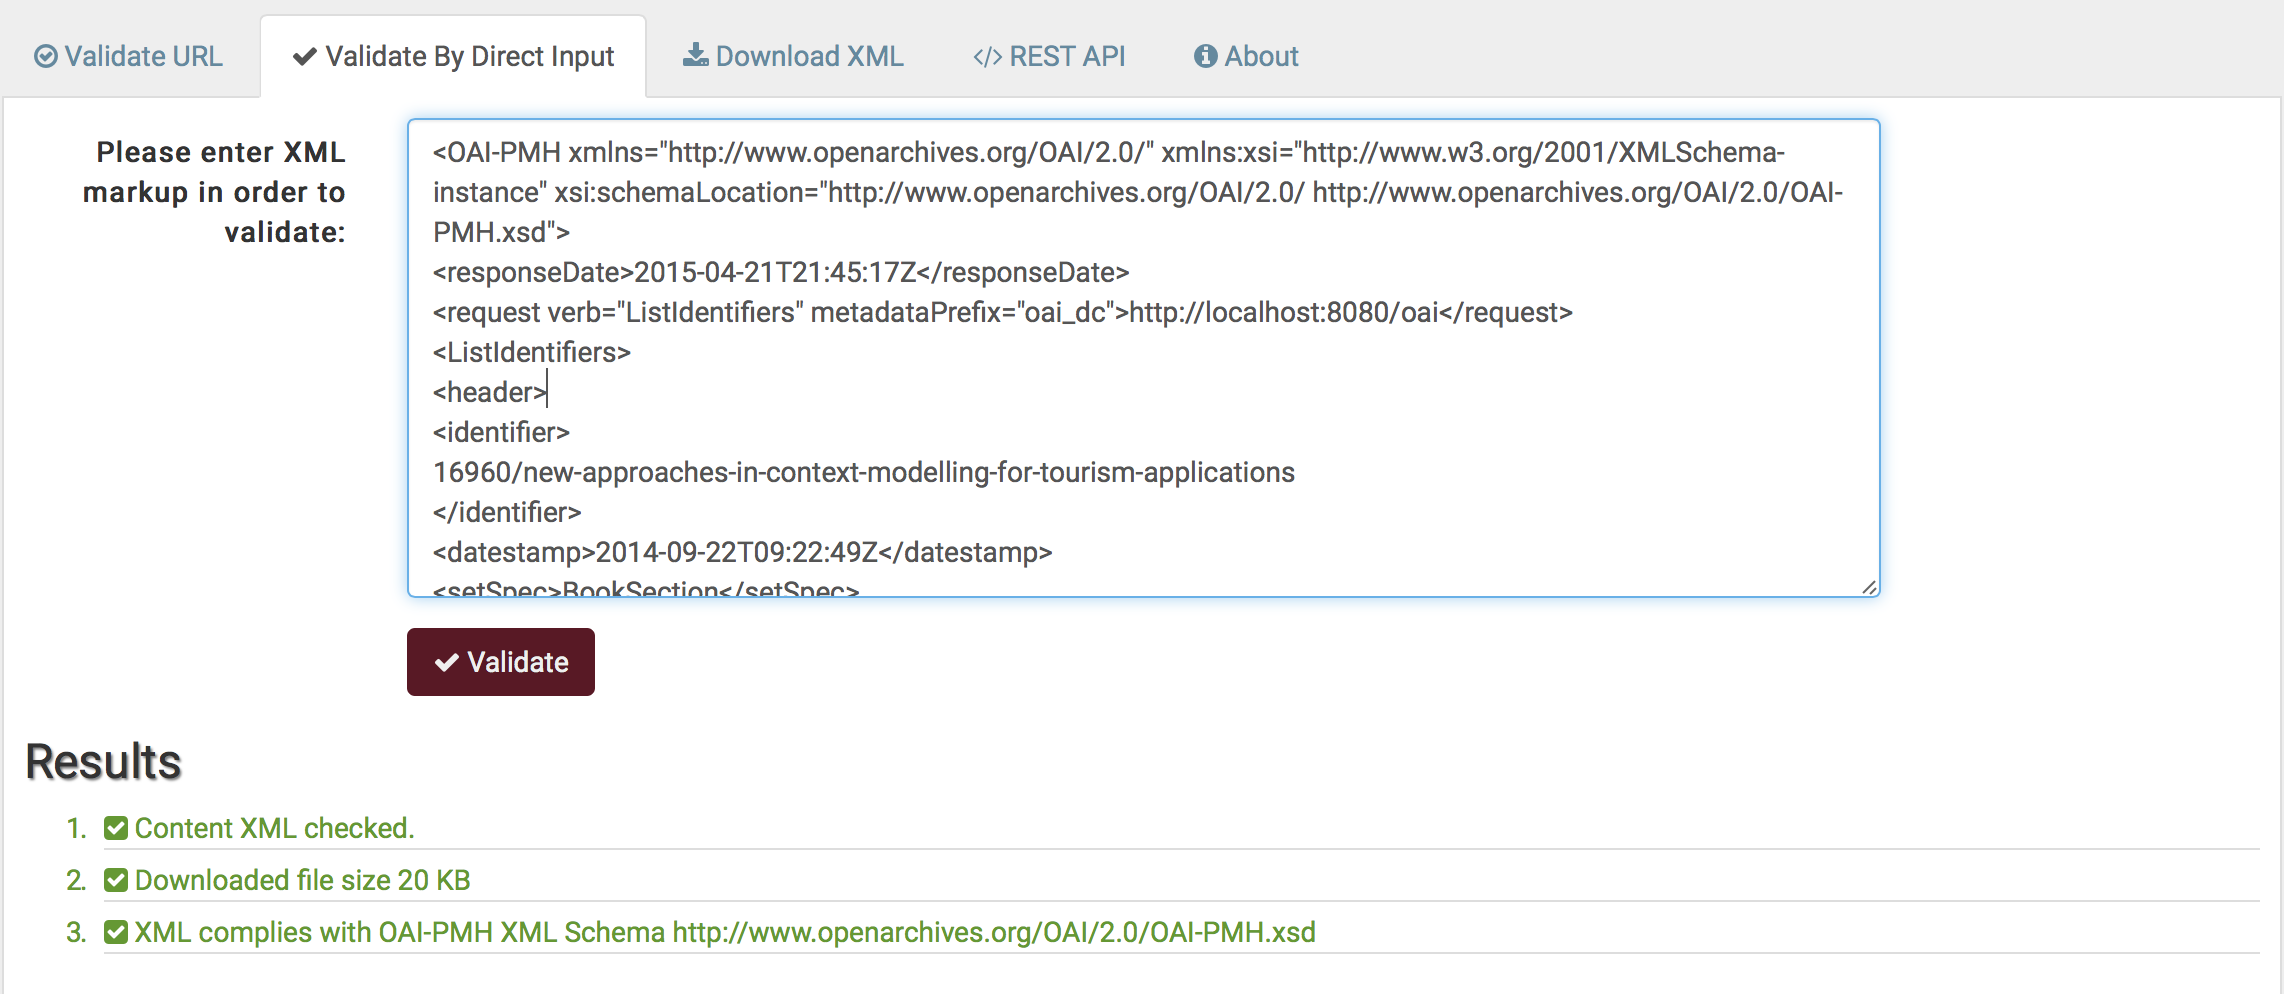
\includegraphics[scale=0.32]{fig/oaipmh_validations/ListIdentifiers}
	\caption{Validación satisfactoria del comando ListIdentifiers}
	\label{fig:listidentifiers}
\end{figure}
